\chapter{Analysis and Design}
\label{chap:analysis-and-design}


\bigskip

\dots We summarize something in Table~\ref{tab:java-advantages}.

\begin{table}[tb] % placement: h for here, t for top, b for bottom
  \centering
  \begin{tabular}{l c}  % two columns: l for left, c for center, r for right
    Feature  & Benefit
 \\\hline
    Objects  & State encapsulation
 \\
    Generics & Code reuse
  \end{tabular}
  \caption{Advantages of Java}
  \label{tab:java-advantages}
\end{table}

\bigskip

\noindent
LaTeX indents a new paragraph unless you specify \lstinline{\noindent}.

\bigskip

We can also refer to Figure~\ref{fig:firefox-js-console}.

\begin{figure}[tb] % placement: h for here, t for top, b for bottom
  \centering
  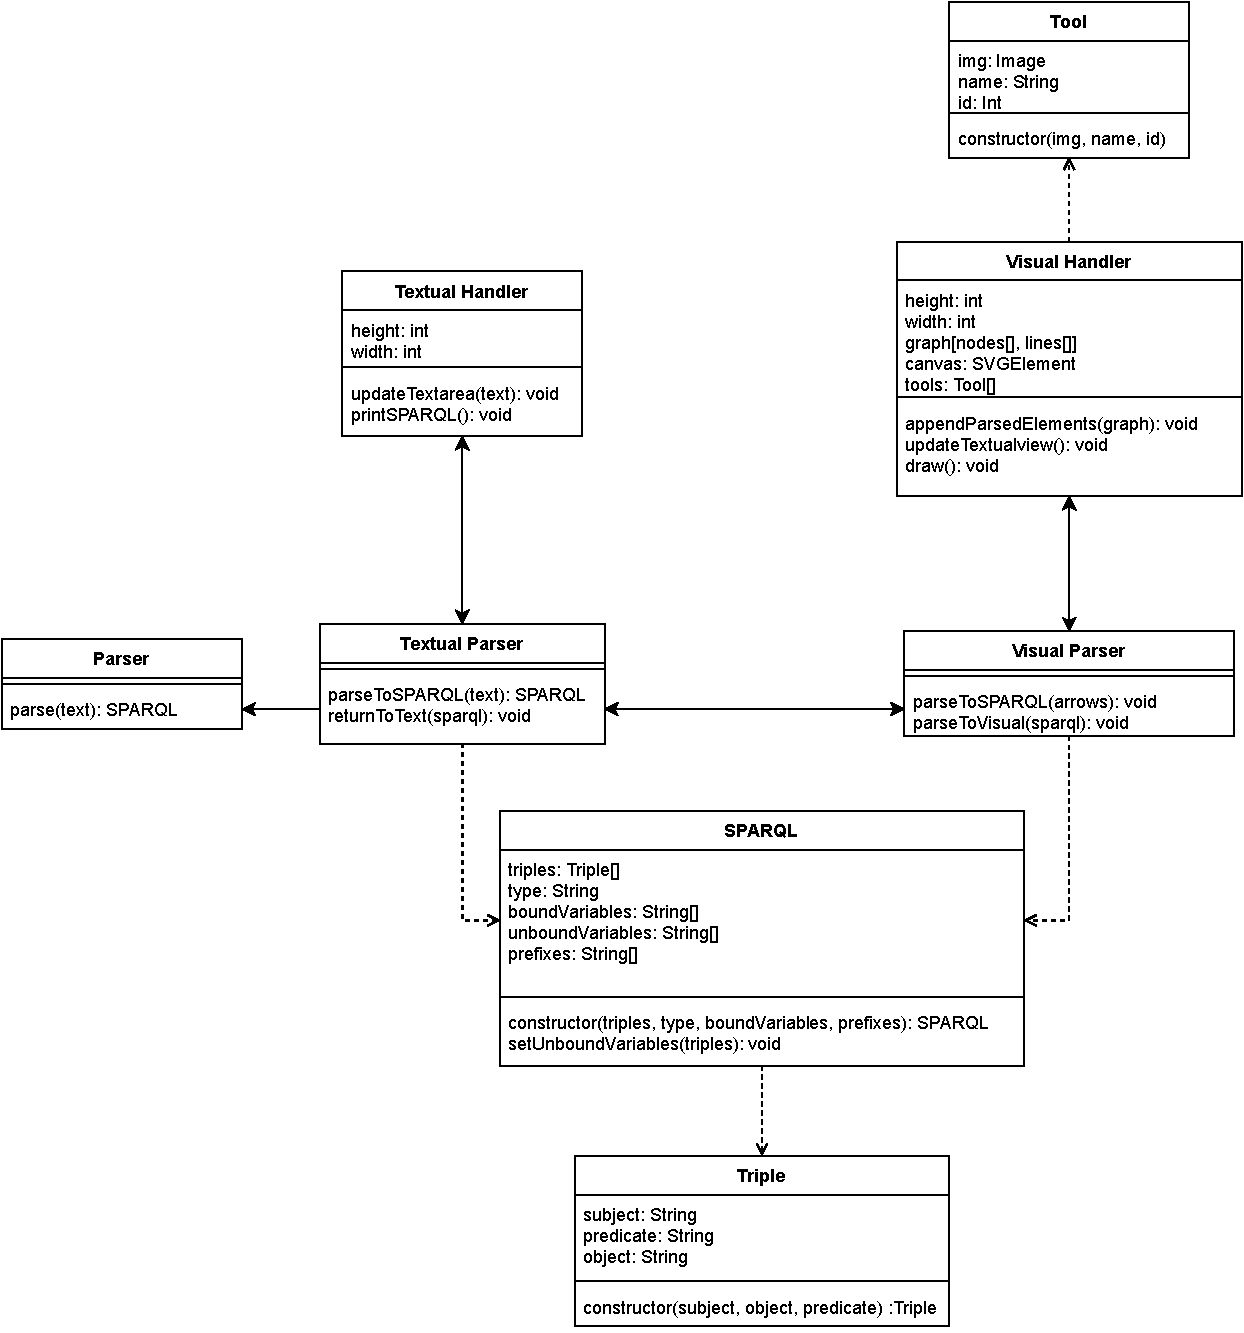
\includegraphics[width=.9\linewidth]{2nd_iteration_design.pdf}
  \caption{The JavaScript console in Firefox }
  \label{fig:firefox-js-console}
\end{figure}
